\documentclass[11pt,a4paper]{article}
\usepackage{fontspec}
\setmainfont{TeX Gyre Pagella}
\newfontfamily\headfont{Inter}[UprightFont=*-ExtraBold,BoldFont=*-ExtraBold,Extension=.otf,Path=/usr/share/fonts/opentype/inter/]
\usepackage[a4paper,margin=2.3cm]{geometry}
\usepackage{graphicx,booktabs,float,caption,array,xcolor}
\usepackage[hidelinks]{hyperref}
\usepackage{titlesec}
\usepackage[round]{natbib}
\usepackage{setspace}
\setstretch{1.05}
\renewcommand{\topfraction}{0.9}
\renewcommand{\bottomfraction}{0.8}
\renewcommand{\textfraction}{0.1}
\renewcommand{\floatpagefraction}{0.75}
\setlength{\parindent}{0pt}
\setlength{\parskip}{0.55em}
\titleformat{\section}{\headfont\Large}{\thesection}{0.8em}{}
\titleformat{\subsection}{\headfont\large}{\thesubsection}{0.8em}{}
\captionsetup{font=small,labelfont=bf}
\urlstyle{same}
\hypersetup{pdftitle={Caravanserais of the Silk Roads: Where the Inns Were, How Far Apart, and Who Built Them},pdfauthor={Tristan Hotham}}

\begin{document}
\begin{center}
{\Large\bfseries Caravanserais of the Silk Roads\par}
\vspace{0.4em}
{\large Where the inns were, how far apart, and who built them:\\an open-data map from Wikidata and OpenStreetMap\par}
\vspace{1.2em}
{\large Tristan Hotham\par}
\vspace{0.3em}
{\small Independent researcher\\
ORCID: 0000-0003-4931-9349\\
DOI: \href{https://doi.org/10.5281/zenodo.24043674}{https://doi.org/10.5281/zenodo.24043674}\par}
\vspace{0.8em}
2026
\end{center}

\begin{quote}
\small
\begin{center}\textbf{Abstract}\end{center}
Caravanserais, the walled roadside inns of the Islamic world and its neighbours, are said to have been built about a day's march apart. I merge the caravanserais, khans and ribats recorded in Wikidata (864 items with coordinates) with the features tagged as caravanserais in OpenStreetMap (281), giving 960 records in 33 countries and territories, of which 953 are inns and 7 are ribats in the sense of forts or Sufi lodges. Turkey (401) and Iran (352) hold 78\%. Grouping inns within 3 km into 727 stops, the median distance from a stop to its nearest neighbour is 20.9 km, well below the 30 to 40 km usually given for a day's stage, and only 12.1\% of gaps fall in that range. Taken one dynasty at a time, the pattern changes: the 90 Safavid caravanserais of Iran stand a median 33.7 km from the nearest other Safavid one (interquartile range 25.7 to 50.1 km). The crowding of the full record is the sum of many building campaigns along the same roads. Only 32.6\% of inns can be given a dynasty, almost all from their architectural style, and 32.6\% carry a heritage listing in Wikidata, mostly in Iran. A hand-inked interactive map accompanies the paper.

\textbf{Keywords:} caravanserai; khan; Silk Roads; Safavid; Seljuk; historical geography; Wikidata; OpenStreetMap; open data; mapping
\end{quote}

\section{Introduction}
A caravanserai (Persian \emph{k\=arv\=ansar\=a}, Turkish \emph{kervansaray} or \emph{han}, Arabic \emph{kh\=an}) is a walled courtyard building that sheltered travellers, their animals and their goods. The type runs from the early Islamic ribats of Central Asia through the great thirteenth century hans of the Seljuk sultans of Rum to the hundreds of caravanserais built along the roads of Safavid Iran, and on to the urban khans of Ottoman and Mamluk cities, where merchants stored and sold goods \citep{erdmann1961,siroux1949,kiani1990,hillenbrand1994,constable2003}. In 2023 UNESCO inscribed fifty-four Iranian caravanserais as the World Heritage Site of the Persian Caravanserai \citep{unesco2023}.

A recurring statement in this literature is that roadside caravanserais were built about one day's march apart, a stage that is often put at 30 to 40 km for laden camels or mules. This is easy to say and hard to check, because there is no open gazetteer of caravanserais. This paper builds one from the two large open sources that record them, Wikidata and OpenStreetMap, and asks three questions: where the recorded caravanserais are; how far apart they stand, and whether that matches a day's march; and what the open record says about who built them and what survives.

The answer to each is shaped by the data as much as by history. I report the record as it is, with its gaps, and present the results as a hand-inked interactive map (\url{https://maps.tristanhotham.com/caravanserais/}) built on The Inked World map engine \citep{inkmap}.

\section{Data}
\textbf{Wikidata.} I queried every item that is an instance of caravanserai (Q186347), khan (Q115921107) or ribat (Q1333989), or of any subclass of them, with coordinates (P625). The query returned 866 items; 2 had only an unknown-value coordinate and were dropped, leaving 864. For each I kept the English label and a label in another language, country (P17), inception (P571) with its precision, architectural style (P149), heritage designation (P1435), number of sitelinks and English Wikipedia article. Wikidata is CC0.

\textbf{OpenStreetMap.} Every node, way and relation tagged \texttt{historic}, \texttt{building}, \texttt{heritage:type} or \texttt{amenity} = \texttt{caravanserai}, through the Overpass API \citep{osm}: 285 features, with their centre points and tags. OpenStreetMap is licensed under the ODbL 1.0, and the derived data that contain it are shared under the same licence. A wider search of OpenStreetMap names (khan, han, ribat, funduq and their equivalents) was planned but its results were not available for this version, so only explicitly tagged features are used.

\textbf{Natural Earth.} 1:10m countries, for the country of each record, and populated places with their population, for the urban rule \citep{naturalearth}.

\begin{table}[tbp]\centering\small\caption{Sources and what was kept.}\label{tab:sources}\begin{tabular}{>{\raggedright\arraybackslash}p{3.2cm}>{\raggedright\arraybackslash}p{6.4cm}r>{\raggedright\arraybackslash}p{2.2cm}}\toprule Source & Kept & Records & Licence\\\midrule
Wikidata & Caravanserais, khans and ribats with coordinates & 864 & CC0\\
OpenStreetMap & Features tagged as caravanserais (after merging duplicates) & 281 & ODbL 1.0\\
Merged & One record per building & 960 & ODbL 1.0\\
Natural Earth & Countries and populated places & & Public domain\\
\bottomrule\end{tabular}\end{table}

\section{Methods}
\subsection{Merging}
OpenStreetMap features were first merged with each other where a node and a way were drawn for one building (within 60 m, 4 cases). A feature was then matched to a Wikidata item through its \texttt{wikidata} tag (116), or, failing that, to the nearest unmatched item within 150 m (69; a second rule allowing 500 m when the names share a word added none). The remaining 96 features are new records; many are unnamed ruins in Afghanistan and Iran. The merged list has 960 records: 679 from Wikidata alone, 185 from both and 96 from OpenStreetMap alone.

\subsection{Kinds and settings}
Seven Wikidata items are ribats in the older sense: frontier forts or Sufi lodges in Tunisia (Monastir, Sousse, Lamta, Sidi Khanfir), Portugal and Spain. They are kept on the map as forts and excluded from all counts of inns. In Iran and Central Asia \emph{rob\=at} names a caravanserai and such buildings stay in. An inn is classed as \emph{urban} if it lies within 2 km of a Natural Earth populated place of 50,000 people or more (3 km for 200,000, 5 km for a million), if two other inns lie within 1 km, or if it belongs to a group of four or more inns linked within 3 km; otherwise it is \emph{roadside}. This gives 698 roadside inns and 255 urban khans. The rule is a rule of thumb: a few town caravanserais in smaller towns are counted as roadside.

\subsection{Stops, spacing and links}
Inns within 3 km of each other (single linkage) are one stop, since a town with several khans was one stage on the road: 727 stops. For each stop I computed the great-circle distance to the nearest other stop. Because a road used for centuries collects inns from many builders, I also measured, for each dynasty, the distance from each inn to the nearest inn of the same dynasty more than 3 km away. To show the chains I took the minimum spanning tree of the stops over the ten nearest neighbours of each and kept edges of 80 km or less, about two days' march. These links are an inference from the positions of the inns, not mapped roads, and straight-line distances understate road distances.

\subsection{Dates and dynasties}
Each inn is given a dynasty from its architectural style in Wikidata where one is recorded (Table~\ref{tab:styles}); if several, the earliest. Otherwise it is given one from the year of building and the region, using conventional dates: in Iran, the Caucasus and Central Asia, before 1040 early, then Seljuk to 1220, Ilkhanid and Timurid to 1501, Safavid to 1736 and Afsharid, Zand and Qajar to 1925; in Anatolia Seljuk from 1075 to 1308 and Ottoman after; in the Levant and Egypt Mamluk from 1250 to 1517 and Ottoman to 1918; in South Asia Mughal and Suri from 1526. A year given only to the century is taken as the middle of that century. Three inceptions are not building dates (a year 11, a Roman site and a museum opening of 2009) and were not used.

\begin{table}[tbp]\centering\small\caption{Architectural styles of inns in Wikidata and the dynasty each implies.}\label{tab:styles}\begin{tabular}{llr}\toprule Style (P149) & Dynasty & Inns\\\midrule
Qajar architecture & Afsharid, Zand and Qajar & 102\\
Safavid architecture & Safavid & 102\\
Ottoman architecture & Ottoman & 65\\
Anatolian Seljuk architecture & Seljuk & 19\\
Seljuk architecture & Seljuk & 9\\
Timurid architecture & Ilkhanid and Timurid & 7\\
Zand architecture & Afsharid, Zand and Qajar & 7\\
Ilkhanid architecture & Ilkhanid and Timurid & 6\\
Shirvan-Absheron school & not used & 6\\
Sasanian architecture & Before the Seljuks & 5\\
Pahlavi architecture & Modern & 2\\
Mamluk architecture & Mamluk & 2\\
Mughal architecture & Mughal and Suri & 2\\
Neoclassical architecture & not used & 2\\
Moorish Revival architecture & not used & 2\\
Damascene architecture & not used & 1\\
Byzantine architecture & not used & 1\\
Islamic architecture & not used & 1\\
Art Nouveau & not used & 1\\
architecture of Iran & not used & 1\\
Ziyarid architecture & Before the Seljuks & 1\\
Ghaznavid architecture & Before the Seljuks & 1\\
\bottomrule\end{tabular}\end{table}

\section{Results}
\subsection{Where they are}
The record is concentrated in two countries: Turkey has 401 records and Iran 352, together 78.4\% (Table~\ref{tab:regions}, Figure~\ref{fig:regions}). The Caucasus, the Levant and Iraq and Central Asia and Afghanistan follow with a few dozen each; South Asia has 17 records, including sarais of the Grand Trunk Road, and China none. In Anatolia 135 of 403 records are urban khans, reflecting the Ottoman hans of Istanbul, Bursa and other cities.

\begin{table}[tbp]\centering\small\caption{Records by region. Inn columns exclude the seven ribats; stops group inns within 3 km; the last column is the median distance to the nearest other stop (km).}\label{tab:regions}\setlength{\tabcolsep}{4pt}\begin{tabular}{lrrrrrrr}\toprule Region & All & Roadside & Urban & Dated & Listed & Stops & Median km\\\midrule
Anatolia & 403 & 268 & 135 & 66 & 1 & 290 & 18.0\\
Iran & 352 & 305 & 47 & 189 & 234 & 299 & 21.5\\
Caucasus & 41 & 22 & 19 & 18 & 29 & 27 & 40.0\\
Central Asia and Afghanistan & 52 & 43 & 9 & 3 & 11 & 39 & 27.3\\
Levant and Iraq & 51 & 25 & 26 & 19 & 8 & 32 & 29.6\\
Egypt and Arabia & 18 & 5 & 13 & 4 & 3 & 7 & 36.8\\
Balkans and Crimea & 17 & 13 & 4 & 8 & 11 & 15 & 91.8\\
South Asia & 17 & 17 & 0 & 4 & 12 & 17 & 19.5\\
Maghreb and Europe & 9 & 0 & 2 & 0 & 2 & 1 & n/a\\
\bottomrule\end{tabular}\end{table}

\begin{figure}[tbp]\centering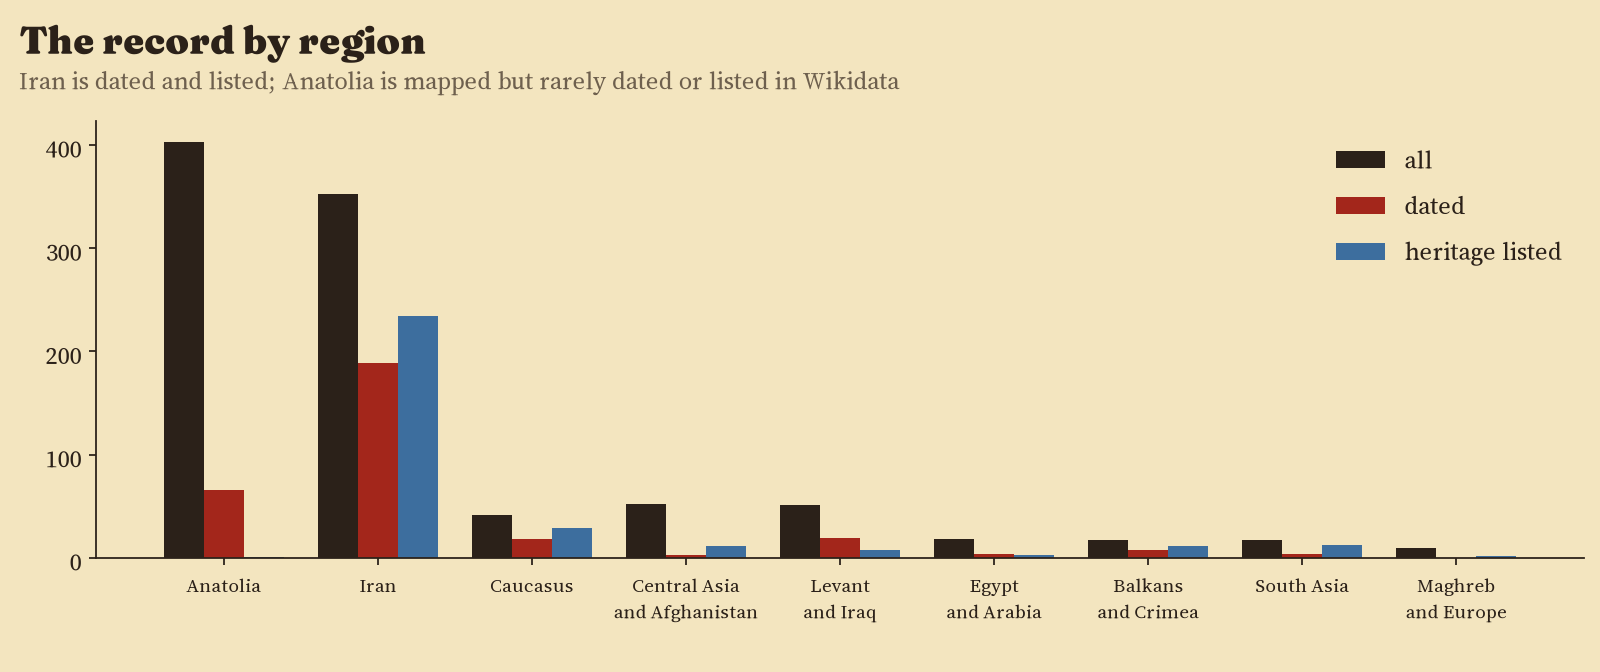
\includegraphics[width=\textwidth]{fig_regions.png}\caption{Records by region: all records, those with a dynasty, and those with a heritage listing in Wikidata.}\label{fig:regions}\end{figure}

The links join 89.7\% of stops into 19 chains of three or more stops, with 646 links totalling 19,031 km. The largest runs for 273 stops across Anatolia, from Çeşme on the Aegean to near Cizre on the Tigris (1,398 km apart in a straight line); the second, of 259 stops, runs across Iran from Gilan on the Caspian to the coast of the Gulf (1,203 km). Figure~\ref{fig:iran} shows the Iranian network on the hand-inked map.

\begin{figure}[tbp]\centering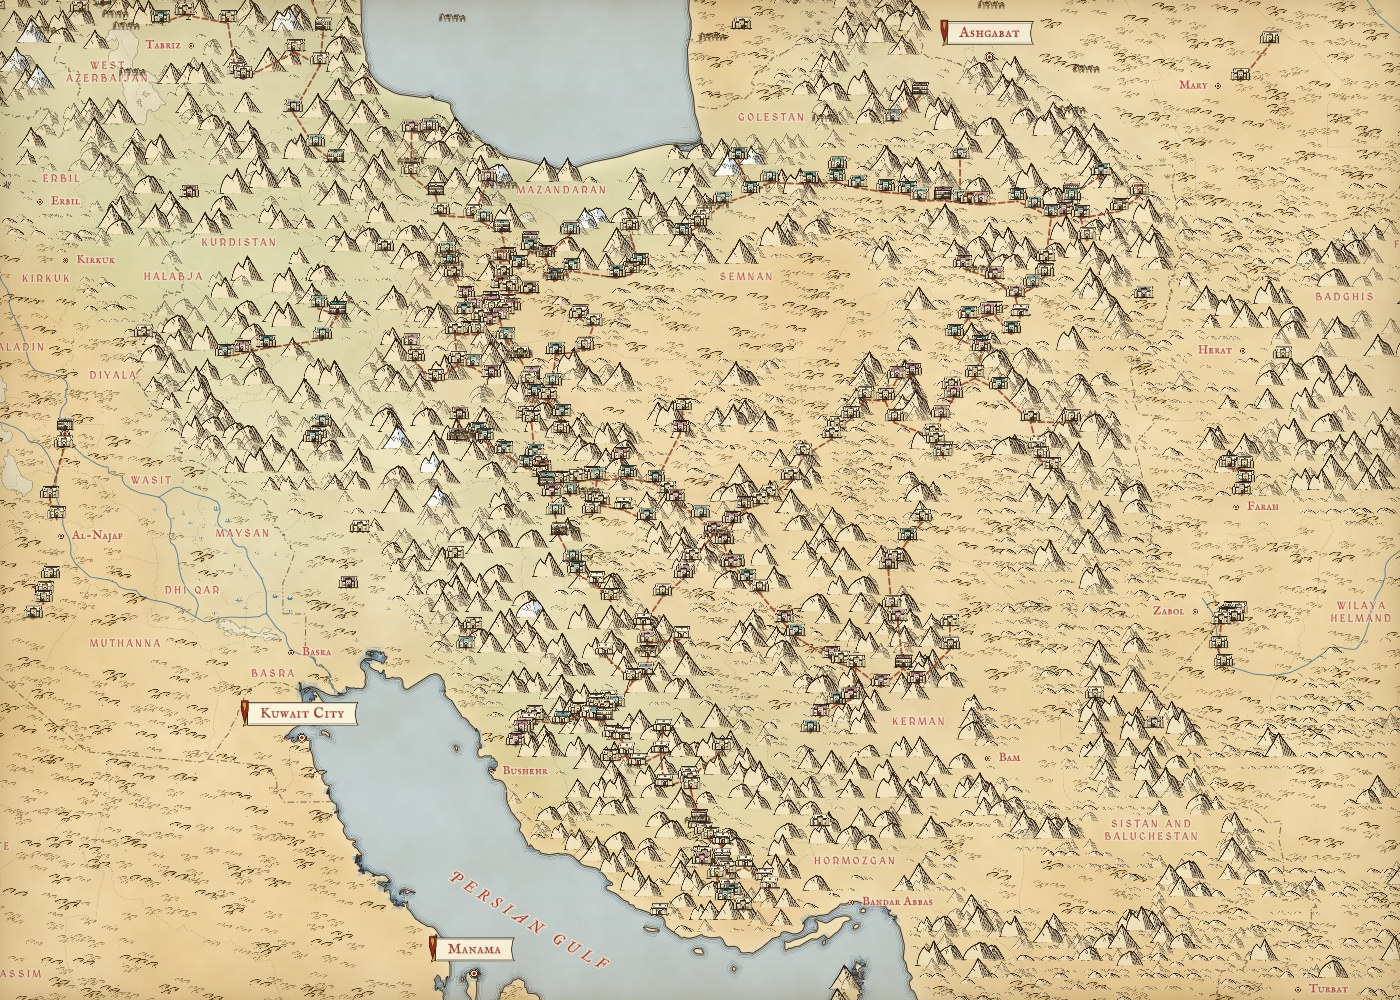
\includegraphics[width=\textwidth]{map_iran.jpg}\caption{Caravanserais of Iran on the hand-inked base map, with the inferred links (dashed). Courtyard colours: turquoise Safavid, rose Afsharid, Zand and Qajar, plain undated.}\label{fig:iran}\end{figure}

\subsection{Spacing}
The median distance from a stop to its nearest neighbour is 20.9 km (interquartile range 12.6 to 35.0 km). Only 12.1\% of gaps lie between 30 and 40 km and 48.3\% are under 20 km (Figure~\ref{fig:spacing}, Table~\ref{tab:spacing}). The medians are similar in Iran (21.5 km) and Anatolia (18.0 km). Link lengths in the spanning tree, which approximate the step from one stop to the next along a chain, have a median of 25.9 km.

One dynasty at a time, the gaps lengthen. The 90 Safavid caravanserais of Iran stand a median 33.7 km from the nearest other Safavid one, with half of the gaps between 25.7 and 50.1 km and 57.8\% between 20 and 50 km: a day's march. The Afsharid, Zand and Qajar inns of Iran are further apart from each other (median 46.4 km), consistent with later builders filling gaps in an existing network rather than laying a new chain. The Seljuk hans of Anatolia (20 with a style or date) and the roadside Ottoman inns there (18) are too few and too incompletely dated to test.

\begin{figure}[tbp]\centering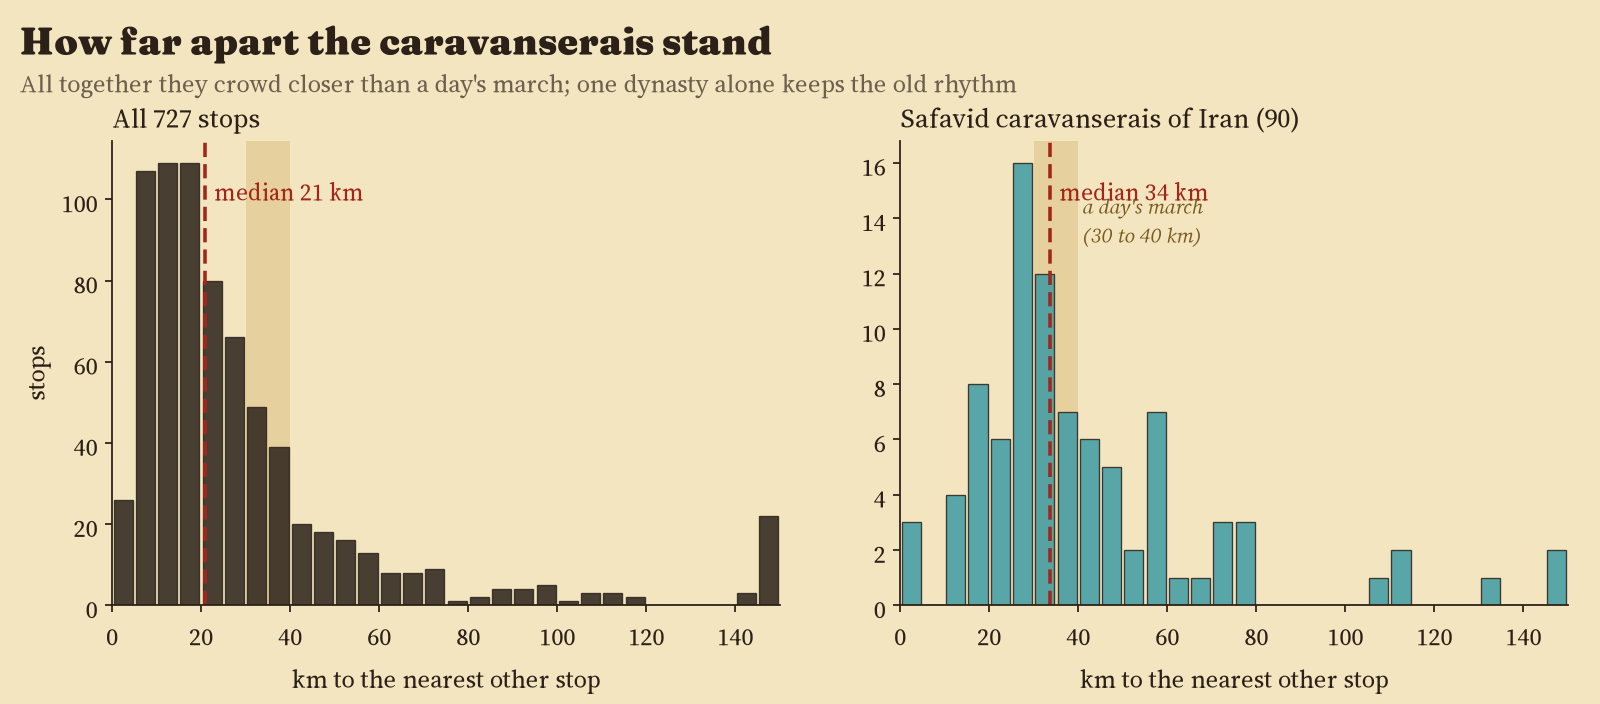
\includegraphics[width=\textwidth]{fig_spacing.png}\caption{Distance from each stop to the nearest other stop (left) and from each Safavid caravanserai in Iran to the nearest other Safavid one (right), in 5 km bins; values above 150 km are drawn in the last bin. The shaded band is a day's march of 30 to 40 km.}\label{fig:spacing}\end{figure}

\begin{table}[tbp]\centering\small\caption{Spacing of caravanserais (great-circle km).}\label{tab:spacing}\setlength{\tabcolsep}{4pt}\begin{tabular}{lrrrrr}\toprule Measure & n & Median & Quartiles & \% 30 to 40 & \% 20 to 50\\\midrule
All stops, nearest neighbour & 727 & 20.9 & 12.6 to 35.0 & 12.1 & 37.4\\
Roadside stops only & 647 & 19.7 & 11.7 to 33.5 & 11.4 & 36.8\\
Links of the spanning tree ($\leq$ 80 km) & 646 & 25.9 & 15.3 to 39.8 & 16.1 & 48.3\\
Safavid inns of Iran, same dynasty & 90 & 33.7 & 25.7 to 50.1 & 21.1 & 57.8\\
Afsharid, Zand and Qajar inns of Iran & 74 & 46.4 & 29.7 to 62.9 & 12.2 & 44.6\\
Seljuk inns of Anatolia & 20 & 46.6 & 19.2 to 70.4 & 5.0 & 35.0\\
Ottoman roadside inns of Anatolia & 18 & 89.5 & 45.9 to 137.1 & 16.7 & 27.8\\
\bottomrule\end{tabular}\end{table}

\subsection{Dates and dynasties}
Only 311 of the 953 inns (32.6\%) can be given a dynasty: 274 from their style and 37 from a year alone. Just 61 have a usable year of building, from 1,050 to 1,896 (Figure~\ref{fig:years}). Safavid is the commonest dynasty (97), then Afsharid, Zand and Qajar (78), Ottoman (70) and Seljuk (29) (Figure~\ref{fig:dynasty}). The Seljuk total is far below the number of thirteenth century Anatolian hans known to scholarship \citep{erdmann1961}: most of the hans in Wikidata carry neither a style nor a date. In 2 cases the style and the year disagree; the style was used.

\begin{figure}[tbp]\centering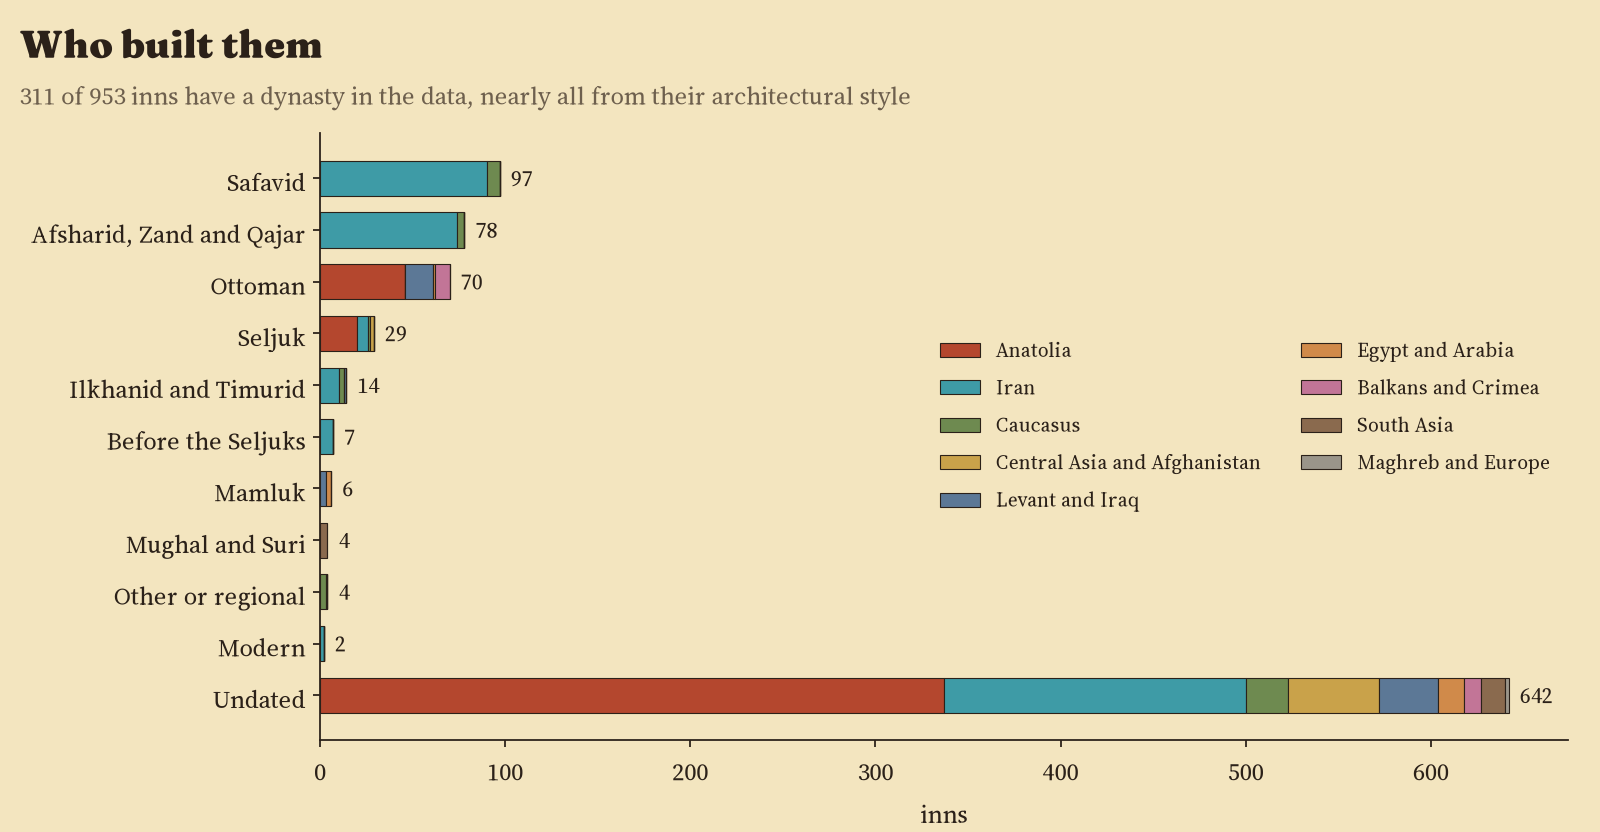
\includegraphics[width=\textwidth]{fig_dynasty.png}\caption{Inns by dynasty, coloured by region.}\label{fig:dynasty}\end{figure}
\begin{figure}[tbp]\centering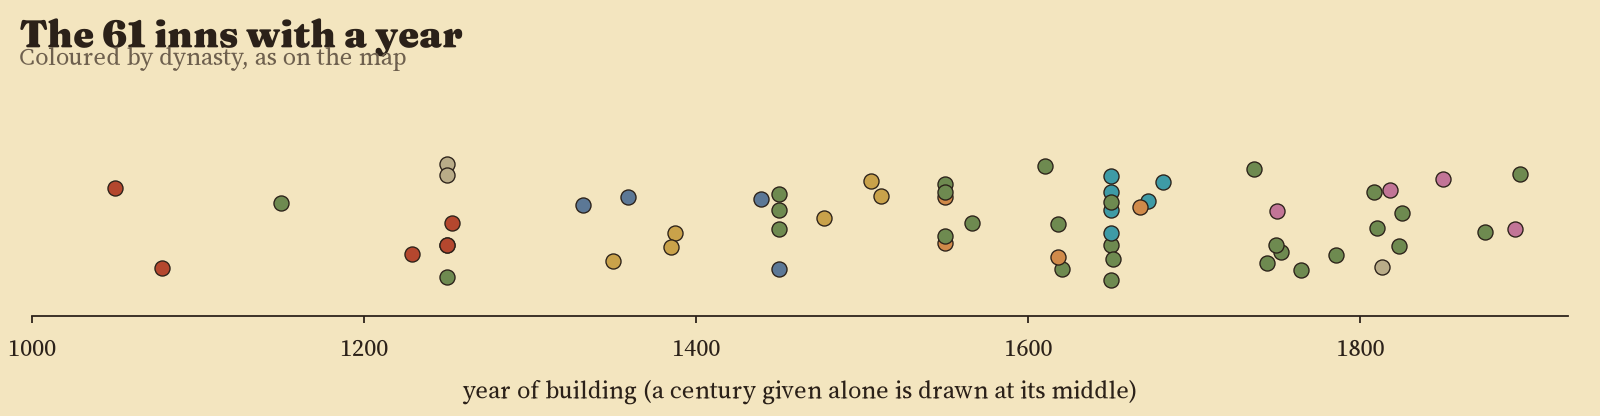
\includegraphics[width=\textwidth]{fig_years.png}\caption{The inns with a year of building, coloured by dynasty; vertical position is random.}\label{fig:years}\end{figure}

\subsection{Heritage and survival}
311 inns (32.6\%) carry a heritage designation in Wikidata: 213 are on the Iranian National Heritage list and 47 are recorded as part of a UNESCO World Heritage Site, almost all of them components of the Persian Caravanserai. In Iran 66.5\% of mapped caravanserais are listed, in Anatolia only 1: Wikidata does not record the Turkish national register for these buildings. OpenStreetMap tags 36 inns as ruins and 17 as reused as hotels, guest houses, museums or restaurants. Figure~\ref{fig:anatolia} shows the Seljuk road through central Anatolia.

\begin{figure}[tbp]\centering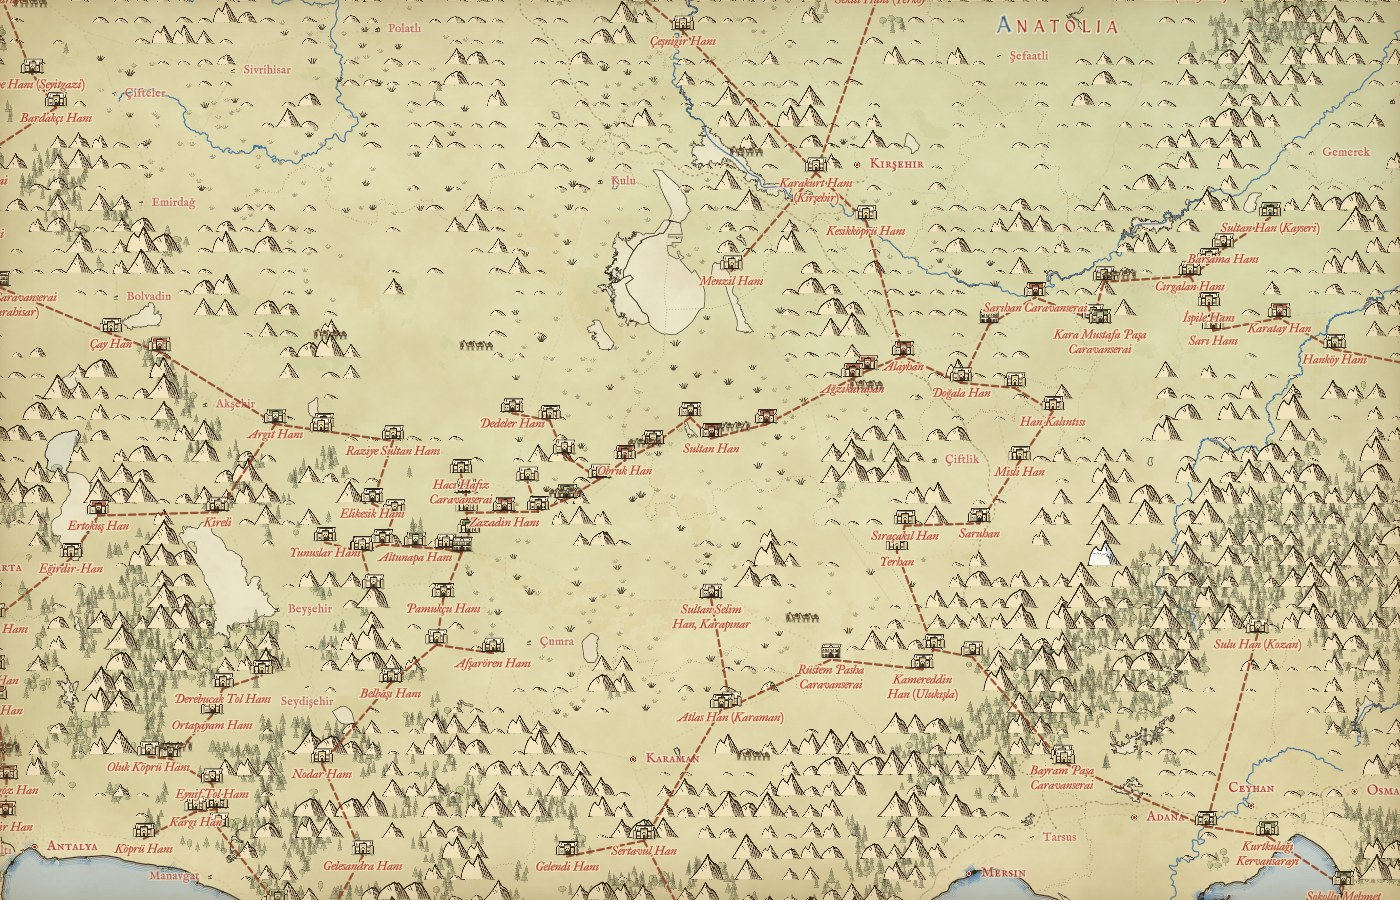
\includegraphics[width=\textwidth]{map_anatolia.jpg}\caption{Central Anatolia between Konya, Aksaray and Kayseri on the hand-inked map. Madder courtyards are Seljuk, olive Ottoman.}\label{fig:anatolia}\end{figure}

\section{Discussion}
The claim that caravanserais stood a day's march apart survives the test, but only once the record is split by builder. A road used from the eleventh to the nineteenth century accumulates inns from several campaigns, and the full set of points is denser than any one network ever was. The Safavid case is the clearest because Safavid caravanserais are numerous, well identified by style and concentrated on a coherent road system; its median spacing of 33.7 km sits inside the 30 to 40 km band. Straight-line gaps understate distances on the ground, so the true stages were somewhat longer.

The geography of the record is a geography of cataloguing. Turkey and Iran are where volunteers and heritage agencies have entered caravanserais into Wikidata, and Iran's national list gives it both coordinates and dates. Central Asia, Arabia, South Asia and China, which had caravanserais on the same scale, are almost absent. Any comparison between regions in this paper is therefore a comparison of records.

\section{Limitations}
The data are incomplete and uneven: many known caravanserais are missing, and some OpenStreetMap features without names may be other ruined buildings. Most inns are undated; architectural style is a proxy for date and may reflect a restoration. The urban rule, the 3 km stop radius and the 80 km link cut-off are choices; other choices change the counts but not the contrast between the full record and one dynasty. Distances are great-circle distances between points. The links and the animated camel trains on the map are illustrations of the inferred network, not reconstructions of roads.

\section*{Data availability}
The merged data (CSV and GeoJSON), the inferred links, all numbers quoted (\texttt{results.json}) and the code are at \url{https://github.com/Tristan-Hotham/caravanserais} and in the Zenodo record of this paper. Data derived from OpenStreetMap are available under the ODbL 1.0; Wikidata content is CC0; code is MIT; text and figures are CC BY 4.0.

\section*{AI assistance}
I wrote the text, with drafting and editing assistance from Claude (Anthropic), which also helped prepare the analysis code. I reviewed and checked all text and results.

\bibliographystyle{plainnat}
\begin{thebibliography}{9}
\bibitem[Constable(2003)]{constable2003} Constable, O. R. (2003) \emph{Housing the Stranger in the Mediterranean World: Lodging, Trade, and Travel in Late Antiquity and the Middle Ages}. Cambridge: Cambridge University Press.
\bibitem[Erdmann(1961)]{erdmann1961} Erdmann, K. (1961) \emph{Das anatolische Karavansaray des 13. Jahrhunderts}. Berlin: Gebr. Mann.
\bibitem[Hillenbrand(1994)]{hillenbrand1994} Hillenbrand, R. (1994) \emph{Islamic Architecture: Form, Function and Meaning}. Edinburgh: Edinburgh University Press.
\bibitem[Hotham(2026)]{inkmap} Hotham, T. (2026) The Inked World: a zoomable hand-inked style world map from open data. Zenodo. \url{https://doi.org/10.5281/zenodo.23860253}
\bibitem[Kiani and Kleiss(1990)]{kiani1990} Kiani, M. Y. and Kleiss, W. (1990) Caravansary. \emph{Encyclopaedia Iranica} IV/7.
\bibitem[Natural Earth(2026)]{naturalearth} Natural Earth (2026) 1:10m Cultural Vectors. \url{https://www.naturalearthdata.com/}
\bibitem[OpenStreetMap contributors(2026)]{osm} OpenStreetMap contributors (2026) OpenStreetMap, via the Overpass API. ODbL 1.0. \url{https://www.openstreetmap.org/copyright}
\bibitem[Siroux(1949)]{siroux1949} Siroux, M. (1949) \emph{Caravansérails d'Iran et petites constructions routières}. Cairo: Institut français d'archéologie orientale.
\bibitem[UNESCO(2023)]{unesco2023} UNESCO World Heritage Centre (2023) The Persian Caravanserai. \url{https://whc.unesco.org/en/list/1668}
\bibitem[Wikidata(2026)]{wikidata} Wikidata (2026) Wikidata, the free knowledge base. CC0. \url{https://www.wikidata.org/}
\end{thebibliography}
\end{document}
